%!TEX root = ../doc.tex
\chapter{User Centered Design}
\label{sec:usercentric}
Als \textit{User Centered Design} werden Prinzipien und Werkzeuge verstanden, welche den Designern, Entwicklern und allen anderen die an der Entstehung eines Produktes, Services oder Prozesses beteiligt sind, helfen die Bedürfnisse und Wünsche des Endbenutzer während der gesamten Entwicklungsphase mit hoher Priorität in den Vordergrund zu stellen. Dieses Framework steht in starkem Kontrast zu herkömmlichen Entwicklungsmethoden bei welchen die Stakeholders zu einem grossen Teil die Ausrichtung, das Aussehen und Verhalten einer neuen Erschaffung bestimmen. Bei diesen älteren Entwicklungsmethoden kam es vermehrt dazu, dass ein Produkt erst bei der Veröffentlichung zum ersten mal die Hände eines Endbenutzer berührte und sich dann als komplett unnütz herausstellte. Der \textit{User Centered Design} Ansatz involviert mögliche Endbenutzer bereits ab den ersten Entwicklungsphasen und fordert dadurch das Zielpublikum zur Mitgestaltung auf. Dadurch werden viele Probleme die bei einer Markteinführung auftreten können, bereits früh entdeckt und behoben. Die Anwendung dieses Frameworks kostet im Gegensatz zu anderen Methoden mehr Zeit und dadurch auch mehr Geld. \textit{User Centered Design} ist eine iterative Methode, welche nach der Durchführung ihrer Teilschritte wieder von vorne beginnt. In Abbildung \ref{fig:usercentereddesign} ist eine mögliche schematische Darstellung des Ablaufs von \textit{User Centered Design}.

\begin{figure}[ht]
	\centering
  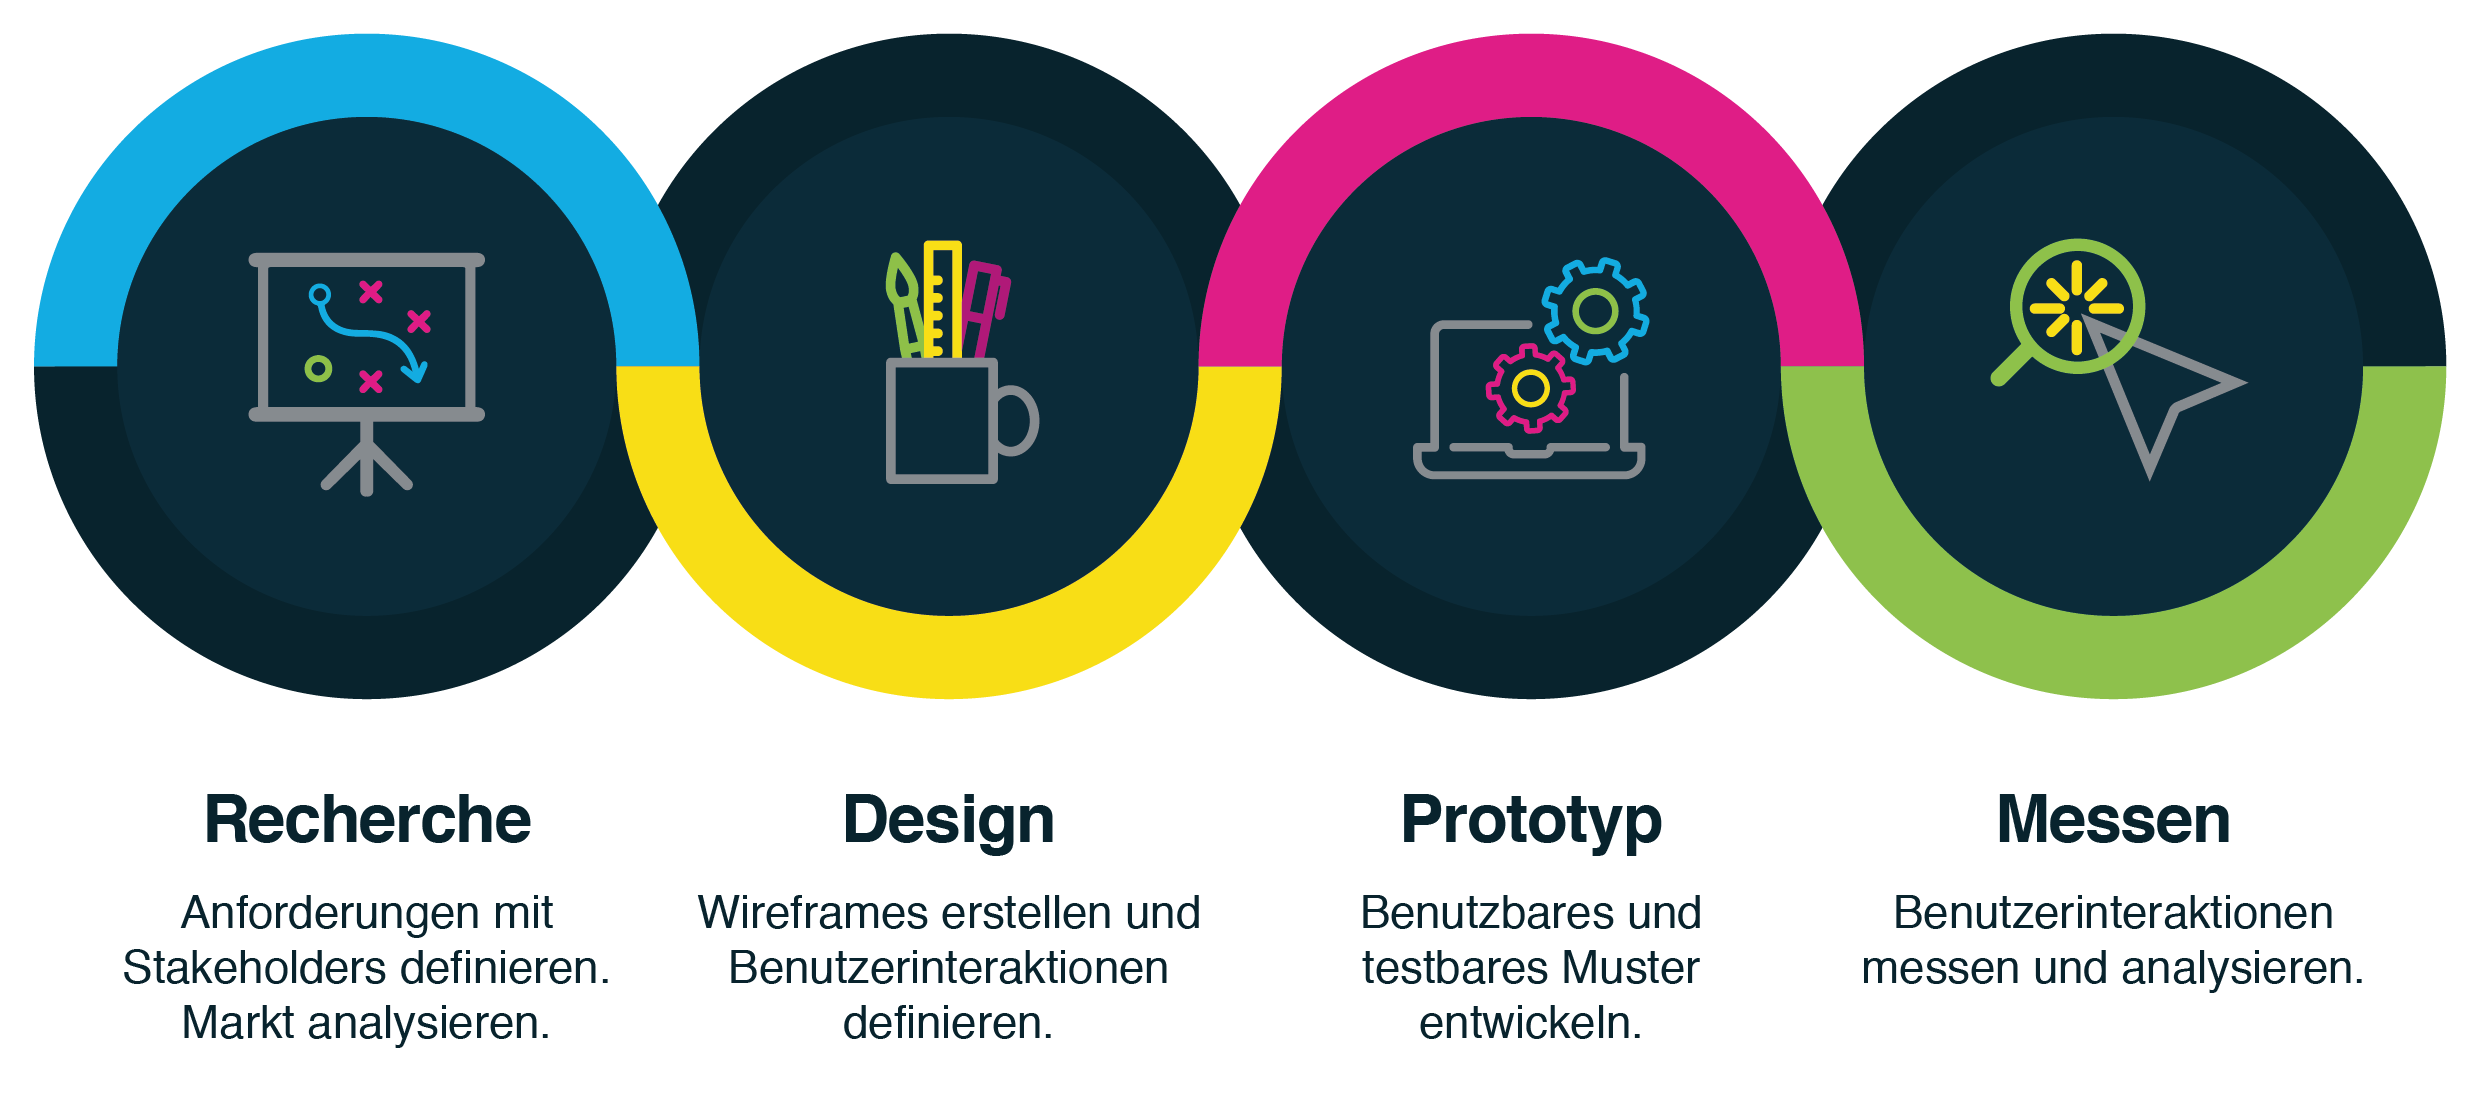
\includegraphics[width=0.88\textwidth]{images/userCenteredDesign.png}
	\caption{Prozessablauf von User Centered Design}
	\label{fig:usercentereddesign}
\end{figure}

Während all diesen Teilschritten werden die Ergebnisse und Erkenntnisse den möglichen Endbenutzern vorgestellt. Dabei wird überprüft ob z.B. der Interaktionsfluss oder die Benutzeroberflächen einer Applikation verständlich ist oder alle relevanten Spezialfälle abdeckt. \textit{User Centered Design} kann auf viele verschiedene Arte angewendet werden und zu den gewünschten Resultaten führen. Diese Bachelorthesis orientiert sich am User Centered Design Ablauf welcher im Buch von Kim Goodwin mit dem Namen \textit{Designing for the Digital Age}\citep{goodwin2011designing} beschrieben wird.


\section{Anwendung}
In den ersten Gesprächen mit den Stakeholdern wurde schnell klar, dass das Ziel des Produktes eine Webapplikation sein soll, welche von Benutzer jeglicher Generation und Demographie benutzt werden kann. Die Entscheidung für eine Entwicklung unter \textit{User Centered Design} war naheliegend. Im folgenden ist der geplante Ablauf mit dem Fokus auf den Endbenutzer beschrieben.

\subsection{Team}
Bei der Zusammenstellung des Design Teams ist es wichtig die verschiedenen benötigten Fähigkeiten in einer kleinen Gruppe zusammen zu fassen. Ein Interaktions Designer hat einen ganz anderen Fokus als der Grafische Designer. Im Rahmen dieser Bachelorthesis fielen alle Rollen des Designs auf eine Person. Diese Konstellation ist nicht per se benachteiligt. Diese einzelne Person muss aber in der Lage sein während den verschiedenen Phasen die Probleme, Ideen, Vorschläge, Lösungen und vieles andere aus den jeweiligen Perspektiven zu betrachten und beurteilen. In der idealen Zusammensetzung nach Goodwin sind folgende Rollen zu besetzen\citep[Kapitel 2]{goodwin2011designing}.
\begin{description}
	\item [Teamleiter\_in] Verantwortlich für das Team und die Koordination mit allen anderen involvierten.
	\item [Interaction Designer\_in (Generator)] Verantwortlich für die Visualisierung des Systemverhalten
	\item [Interaction Designer\_in (Synthesizer)] Verantwortlich für die Analyse und Kommunikation des Designs.
	\item [Grafischer Designer\_in] Verantwortlich für die Visuelle Umsetzung des Designs.
	\item [Industrie Designer\_in] Verantwortlich für das Design der Hardware.
\end{description}

\subsection{Grundlegende Recherche der Domäne}
Während der Recherche wird die Domäne in welcher sich das zu erschaffende Produkt befindet analysiert. Dabei werden Marktanalysen getätigt sowie falls vorhanden die Produkte der Konkurrenz untersucht. Zusätzlich werden Experten und Menschen welche bereits lange in dem Bereich tätig sind befragt. Diese Arbeit wird vom gesamten Design Team bewältigt da bereits in dieser Phase die verschiedene Perspektiven wichtig sind. Mit Nick Blake als Gründer von Imagine Cargo und Experte der Kurier-, Express- und Paketdienst Industrie hat diese Bachelorthesis auf sehr viel Erfahrung und Insiderwissen zurückgreifen können.

\subsection{Interviews mit Stakeholders}
Bevor Interviews beginnen können müssen die Stakeholders zuerst definiert werden. Zu den Stakeholders gehören grundsätzlich alle Menschen die ein Produkt mit bestimmen können. Jedoch zählt nicht jede Meinung gleich viel. Bei der Analyse ist es wichtig mit allen involvierten Menschen zu reden und auch die Personen ausfindig machen, welche sich aus dem ganzen Design Prozess raus halten aber die Macht haben das ganze Projekt zu beerdigen. Üblicherweise finden sich solche Stakeholders im Management die das Gefühl haben ihre Meinung sei noch nicht notwendig bzw. er/sie werde erst aktiv wenn das Projekt ein Fundament hat. Meist ist es dann aber zu spät für Grundlegende Designänderungen. Für die Bachelorthesis wurden David Emmerth und Nick Blake von Imagine Cargo interviewt. Die Fragen für die Interviews sind vom Buch von Kim Goodwin inspiriert worden\citep[Kapitel 5]{goodwin2011designing} und sind im Anhang \ref{subsec:stakeholderfragen} zu finden. Die Zusammenfassungen der Interviews sind in Kapitel \ref{sec:interviews} nach zu lesen.

\subsection{Interviews mit Endbenutzer}
In den Interviews mit den Stakeholdern sollte sich eine grobe Definition des zu erstellenden Produktes heraus kristallisieren. Mit dieser gewonnen Definition werden mit möglichen Endbenutzern Interviews geführt, welche weitere Einblicke in die Anforderungen und Unzufriedenheiten mit bestehenden Produkten zu Tage bringt. Aufgrund der beschränkten Ressourcen die dieser Bachelorthesis zur verfügung stehen, wurde auf diesen Schritt verzichtet. In der Visualisierungs Phase sollen die erstellten Wireframes und den Interaktionsablauf mit möglichen Endbenutzern überprüft werden.

\subsection{Personas}

%Personas erstellen \\
%Persona Stories erstellen & Anforderungen definieren \\





\section{Interviews}
\label{sec:interviews}
\textcolor{darkgray}{
	Beschreibung der geführten Interviews und den Gesprächspartnern
}